% Pacotes e configurações padrão do estilo "article"\
% -------------------------------------
\documentclass[a4paper,12pt]{article}
% Layout
% --------------------------------------------------------------------------------
\usepackage{pdfpages} % Pacote para inserir um PDF dentro do LaTeX
\usepackage{minted} % Pacote para Colorir Código
\usepackage{circuitikz}
\usepackage{verbatim}
%     Gráficos e layout ----------------------------------------------------------------------
\ifx\pdfmatch\undefined
\else
    \usepackage[T1]{fontenc}
    \usepackage[utf8]{inputenc}
\fi
% xetex:
\ifx\XeTeXinterchartoks\undefined
\else
    \usepackage{fontspec}
    \defaultfontfeatures{Ligatures=TeX}
\fi
% luatex:
\ifx\directlua\undefined
\else
    \usepackage{fontspec}
\fi
% End engine-specific settings

%      Fonte --------------------------------------------------------------------------------
%\usepackage{lmodern}
\usepackage{times}
%     Pacotes adicionados -------------------------------------------------------------------
\usepackage{ae}
%     Língua e hifenização ------------------------------------------------------------------
\usepackage[english]{babel}
\usepackage{hyphenat}
% ---------------------------------------------------------------------------------------
\usepackage{fancyhdr}
\usepackage{sectsty}
\usepackage{float}
%\usepackage{graphicx}
%\usepackage[pdftex]{color,graphicx}
\usepackage{hyperref}
\usepackage{enumerate} % Permite alterar Layout do enumerate
%\usepackage{pdflscape} % Permite alterar a orientação da pagina
%\usepackage{ifthen} % Permite usar condicionais ifelse
%\usepackage[table]{xcolor} % Permite alterar as cores das celulas de uma tabela
\usepackage{amsmath,amssymb} % Ambiente para uso de elementos matemáticos
\usepackage{caption}
\usepackage{subcaption} % permite o uso de multiplas figuras com legenda
%     Dados do título e autores --------------------------------------------------------------
%\title{\tituloRelatorio}
\author{Rafael Lima}
%     Definições do pdf ----------------------------------------------------------------------
\hypersetup{
    unicode=false,          % non-Latin characters in Acrobat’s bookmarks
    pdftoolbar=true,        % show Acrobat’s toolbar?
    pdfmenubar=true,        % show Acrobat’s menu?
    pdffitwindow=false,     % window fit to page when opened
    pdfstartview={FitH},    % fits the width of the page to the window    
    pdfauthor={Rafael Lima},     % author
    pdfnewwindow=true      % links in new window
}
% Layout do documento ------------------------------------------------------------------------
 \pagestyle{fancy}
%     Cabeçalho e Rodapé ---------------------------------------------------------------
      \lhead{}
      \chead{}
      \rhead{}
      \lfoot{}
      \cfoot{}
      \rfoot{\thepage}
      %     Númeração ------------------------------------------------------------------------
      \pagenumbering{arabic}
      %     Retas do cabeçalho e rodapé ------------------------------------------------------
      \renewcommand{\headrulewidth}{0.5pt}
      \renewcommand{\footrulewidth}{0.5pt}
      %     Tamanho da letra de seções e derivadas --------------------------------------------
      \sectionfont{\normalsize}
      \subsectionfont{\small}
      %     Hiperlinks ------------------------------------------------------------------------
      \hypersetup{
                  colorlinks,
                  citecolor=black,
                  filecolor=black,
                  linkcolor=black,
                  urlcolor=black
                  }
%     Outros ----------------------------------------------------------------------------
      \addto\captionsbrazilian{\renewcommand{\contentsname}{Índice}} % Muda nome dos contents
      %\renewcommand{\thesection}{(\alph{section})} % muda o estilo de númeração das sections
      % alterando a formatação dos numeradores de lista de itens
      \renewcommand\theenumi{\arabic{enumi}}
      \renewcommand\labelenumi{(\textit{\theenumi})}
	  \renewcommand\theenumii{\arabic{enumii}}
	  \renewcommand\labelenumii{(\textit{\theenumi.\theenumii})}
      
% ---------------------------------------------------------------------------------------

\newcommand{\tituloRelatorio}{Jornal Entry - Class 1}
\title{\tituloRelatorio}
\hypersetup{pdftitle={\tituloRelatorio}}% title

\usepackage{listings}
\lstset{
  language=Matlab,
  basicstyle=\ttfamily\small,
  keywordstyle=\color{blue},
  stringstyle=\color{verde},
  commentstyle=\color{red},
  extendedchars=true,
  showspaces=false,
  showstringspaces=false,
  numbers=left,
  numberstyle=\tiny,
  breaklines=true,
  backgroundcolor=\color{green!10},
  breakautoindent=true,
  captionpos=b,
  xleftmargin=0pt,
}
% Definições Auxiliares
% -----------------------------------------------------------------
%\input{relat_aux.tex}
% ----------------------------------~>ø<~---------------------------------------
\begin{document}
% Capa e Índice ---------------------------------------------------------------
\includepdf[pages=-]{Capa4.pdf}
\newpage
\tableofcontents
\thispagestyle{empty}
% Conteudo -------------------------------------------------------------------
\newpage

\section{Introdução}
O objetivo deste experimento é realizar uma análise no domínio da frequência de um sistema mecânico rotacional controlado por um circuito DC. A fim de realizar esta

\section{Fundamentação Teórica}
Uma análise comumente realizada em sistemas dinâmicos é compreender o comportamento no domínio da frequência do que estamos analizando. Para tanto, podemos usar de várias ferramentas matemáticas para traduzir o equacionamento do domínio do tempo para este novo domínio, tais quais a transformada de Fourier e a transformada de Laplace. Usando, por exemplo, a transformada de Laplace, podemos obter a \textit{função de transferência}. Com a função de transferência em mãos, podemos determinar quais as mudanças que o nosso sistema causará a uma dada entrada.

No nosso caso, estamos trabalhando com sistemas lineares e invariantes no tempo, portanto somente haverá efeitos na magnitude e na fase do nosso sinal (NISE, 2010). Mais precisamente, teremos
\begin{itemize}
    \item um ganho na magnitude, que será um fator multiplicativo em termos da frequência da entrada.
    \item um ganho de fase, que será um fator somador também em termos da frequência da entrada.
\end{itemize}
Consequentemente, podemos rescrever nossa função de saída em termos da frequência. Supondo que a entrada seja algo da forma: $$ u(t) = A e^{\jmath \phi} $$ então a saída será $$ y(t) = A M(\omega) e^{\jmath (\phi + \phi (\omega))}$$ se escrevermos as funções de entrada e saída no formato exponencial.

Falar das aproximações assintóticas do diagrama de bode.

\section{Materiais}
Neste experimento, os seguintes materiais foram utilizados:

\begin{itemize}
    \item Planta servo de movimento rotatório SRV02;
    \item Placa de aquisição de datos: Quanser Q8-USB;
    \item Módulo de potência: Quanser VoltPAQ;
    \item Programa de controle em tempo real: QUARC-Simulink.
\end{itemize}

\section{Procedimentos}
Os procedimentos executados durante o experimento são descritos pelos items seguintes.

\begin{enumerate}
\item Primeiramente, no ambiente \textit{Simulink} do \textit{software} Matlab, o modelo \textit{bode\_srv02.mdl} foi aberto. Este modelo consiste em dois blocos principais, um referente à modelagem real da planta servo de movimento rotatório e o outro, a sua modelagem teórica. O sinal de entrada deste modelo é uma senóide de fase nula e frequência e amplitude ajustáveis. O modelo \textit{bode\_srv02.mdl} pode ser visto na Figura \ref{fig:planta}.

\begin{figure}[H]
\centering
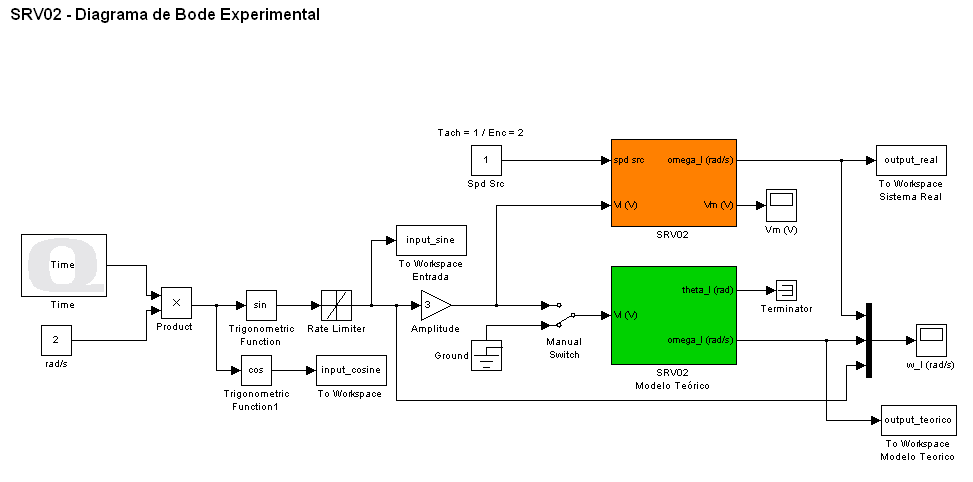
\includegraphics[width=12cm]{img/planta}
\caption{Diagrama de blocos do \textit{Simulink} tirado do modelo \textit{bode\_srv02.mdl}}
\label{fig:planta}
\end{figure}

\item Depois, o \textit{script} \textit{setup\_lab\_srv02\_bode.m} foi executado para que os valores dos parâmetros utilizados pelo modelo aberto no \textit{Simulink} fossem corretamente carregados.

\item Assim, o \textit{script} \textit{bode\_plot.m} foi executado e um diagrama foi gerado. Esse diagrama foi, então, comparado com as expectativas teóricas descitas na secção ``Fundamentação Teórica'' deste relatório.

\item A partir da variação de frequência do sinal de entrada (alteração do valor mostrado no bloco de legenda ``rad/s'') e para uma amplitude defiida por 3, o sistema foi executado em tempo real e os valores de amplitude e fase foram registrados na Tabela \ref{tab:resultados} da secção ``Resultados Experimentais'' deste relatório. Para calcular a amplitude e fase, foi utilizado o \textit{script} \textit{amp\_fase.m}, que retorna a amplitude em decibéis (dB) e a fase em graus. A frequência do sinal de entrada foi variada de tal forma a adquirir os seguintes valores: 1,2,3,4,5,6,7,10,15,20,30,40,60,80 e 100 rad/s.

\item Por fim, cada ponto de amplitude e fase obtidos no item anterior foi plotado nos respectivos diagramas de Bode teóricos. Os comandos utilizados para o diagrama de Bode da amplitude foram \textit{subplot(2,1,1); semilogx(w,M,’o’);} hold on; e para a fase foram \textit{subplot(2,1,2);
semilogx(w,phi,’o’); hold on;} em que \textit{w} representa a frequência de entrada do sistema, \textit{M} é a amplitude de saída e \textit{phi}, sua fase.

\end{enumerate}

\section{Resultados Experimentais}

Resultados aqui.

\begin{table}[H]
    \centering
    \begin{tabular}{|c|c|c|c|}
        \hline
        Frequência (rad/s) & Amplitude da senóide & Amplitude M (dB) & Fase $\phi$ (graus)\\
        \hline
        1 & 3 & 5.2035 & -4.1777 \\
        \hline
        2 & 3 & 4.9145 & -4.5383 \\
        \hline
        3 & 3 & 4.8184 & -4.7945 \\
        \hline
        4 & 3 & 4.8167 & -7.3805 \\
        \hline
        5 & 3 & 4.3704 & -7.7942 \\
        \hline
        6 & 3 & 4.2569 & -9.0500 \\
        \hline
        7 & 3 & 4.3936 & -10.5826 \\
        \hline
        10 & 3 & 4.5397 & -15.5095 \\
        \hline
        15 & 3 & 4.1022 & -23.0883 \\
        \hline
        20 & 3 & 3.6786 & -29.6863 \\
        \hline
        30 & 3 & 2.5258 & -40.6481 \\
        \hline
        40 & 3 & 1.4162 & -48.8259 \\
        \hline
        60 & 3 & -0.7629 & -61.3640 \\
        \hline
        80 & 3 & -2.6985 & -71.0645 \\
        \hline
        100 & 3 & -4.2682 & -77.7609 \\
        \hline
    \end{tabular}
    \caption{Resultados de amplitude e fase para a saída do sistema com entradas de frequências variadas}
    \label{tab:resultados}
\end{table}

\begin{figure}[H]
\centering
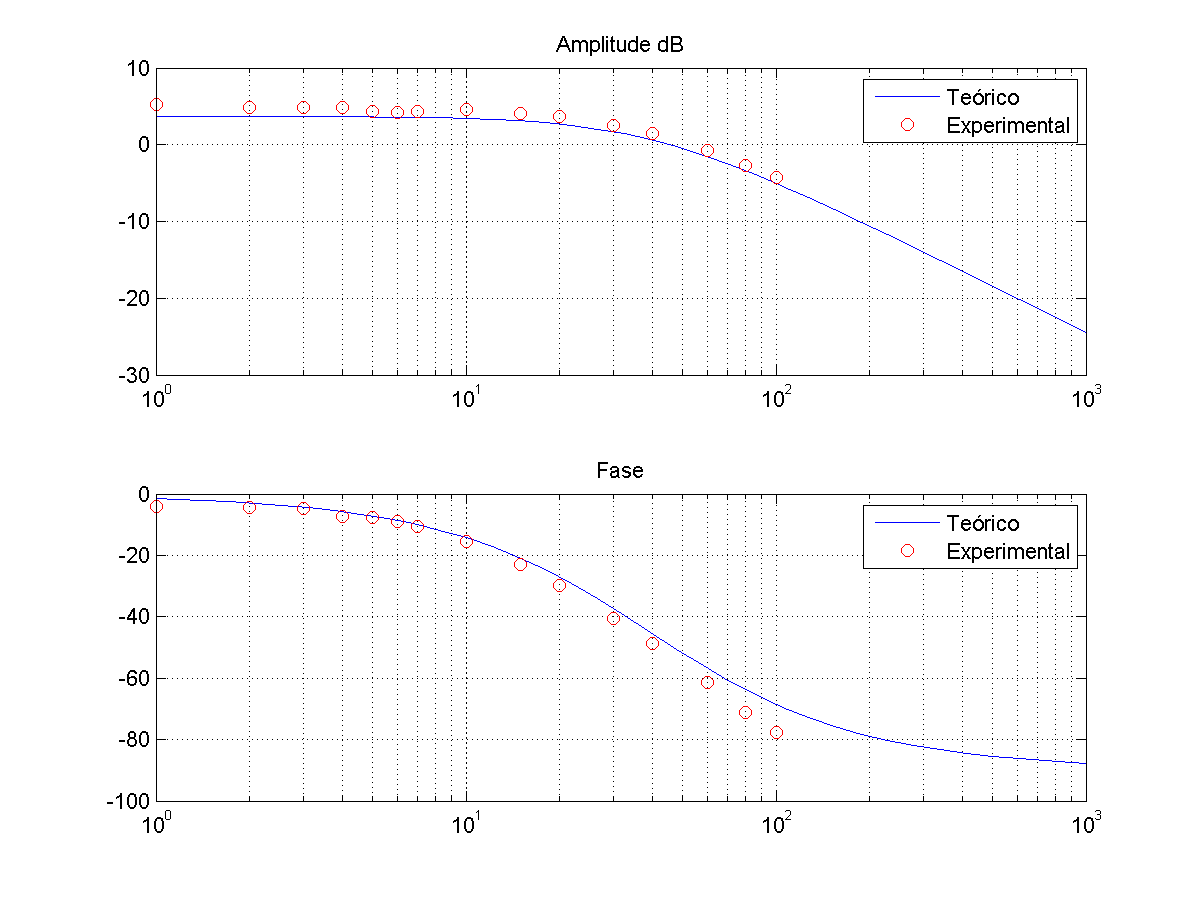
\includegraphics[width=12cm]{img/bode_exp4}
\caption{Diagrama de bode}
\label{fig:bode}
\end{figure}


\section{Exercícios para o relatório e Análise de Dados}
Nesta secção, algumas questões referentes ao experimento realizado são propostas. Essas questões serão respondidas na secção seguinte e formarão a base para a análise dos dados obtidos e registrados na secção de Resultados Experimentais deste relatório.

\begin{enumerate}
    \item Apresente os diagramas de Bode de magnitude e fase obtidos teoricamente e experimentalmente (no mesmo gráfico) e discuta sobre o procedimento para obtenção deles. Avalie a precisão e a qualidade dos diagramas obtidos apresentando algumas razões para eventuais diferenças entre o real e o teórico.
    \item  Uma vez obtidos os diagramas de Bode experimentalmente, explique como seria possível obter um modelo para a planta analisada.
    \item  Discuta eventuais problemas enfrentados durante o experimento e como eles foram solucionados.
\end{enumerate}

\subsection{Respostas dos Exercícios para o relatório (Análise de Dados)}
\begin{enumerate}
    \item 1
    \item 2
    \item 3
\end{enumerate}

\section{Conclusão}

Conclusão aqui.

\begin{thebibliography}{8}
\bibitem{NISE}
Nise N.S.
\emph{Control Systems Engineering} Wiley. 6ª edição. 14 de Dezembro de 2010. 944 páginas.

\bibitem{Quanser}
Quanser,
\emph{Rotary Servo Base Unit}
Disponível em: \url{http://www.quanser.com/products/rotary_servo}
Acesso em: 6 de Setembro de 2016

\bibitem{Manual}
Quanser,
\emph{SRV02 User Manual}
Disponível em: \url{http://www2.hawaii.edu/~gurdal/EE351L/srv02.pdf}
Acesso em: 7 de Setembro de 2016


\end{thebibliography}
% ---------------------------------------------------------------------------------------
\end{document}
